\section{Background}
\label{sec:background}
This chapter will explain some elements to be able to understand the contents of this scientific report.
The focus will be put on graph theory and genetic algorithms.
For both of these the basics will be shortly mentioned and the reasoning behind why they are important for this work.

\subsection{Graph Theory}
Graph theory is the mathematical theory of the properties and applications of graphs.
A graph $G=\left[V,E\right[$ is a collection of vertices (points) and edges (lines).
An edge connects two vertices or creates a loop for one vertice.
Graphs can have a certain properties, e.g. directed, undirected, weighted or complete.
Certain combinations of these properties are also possible.

In directed graphs an edge has an orientation, e.g. $A \rightarrow B$. This says that A has a connection to B, but B does not have a connection to A.
Normally in an undirected graph an edge might look like $A - B$, which implies a connection in both ways.

Edges in the graph can contain a certain scoring-function, if this is the case then it's called a weighted graph.
An common example of this is the euclidean distance between the two vertices the edge connects together.
A graph is complete when all nodes are connected to eachother.
A graph $G'=\left[V',E'\right[$ is a subgraph of $G$ if $V' \subset V$, $E' \subset E$ and $E'$ only including edges between the vertices of $V'$.
A complete subgraph is called a \textbf{clique}.
There are other properties for graphs, but they are not required for the understanding of this report.

\subsection{Genetic Algorithm}
In this subsection the concept of genetic algorithms will be expanded upon. 
First, the basic concept will be explained. 
Afterwards a more concrete explanation will be given about the elements that have been used in this research.
Important to note is that if a problem can be represented and the proper operators can be designed any problem can be solved by a genetic algorithm if the purpose of it is to optimize a certain scoring function.

\subsubsection{Basics}
A genetic algorithm is a metaheuristic inspired by natural evolution and selection.
The goal of the metaheuristic is to mimic biological evolution, which strives to improve on itself.
It is a method for solving optimization problems which can be constrained or unconstrained.
A population of individuals is generated each generated each iteration.
The strongest individual, according to the fitness function, approaches an optimal solution for the given problem.

A typical genetic algorithm contains a genetic representation of the solution domain and a fitness function to evaluate the solution in the problem domain.
The chromosome\footnote{Also known as the genotype.} is the set parameters which define a solution for the problem.
A set of chromosomes is called a population.
By iteratively updating the population by using certain operators, the algorithm attempts to find the optimal solution for the specified problem.

\subsubsection{Representation}
The most commonly used representation in genetic algorithms is the binary representation.
But this isn't always a good choice, because the translation to a representation that we can easily understand (phenotype) might be very difficult.
That is why for the problem that will be discussed in this report we will be using a locus based representation.
An example of this can be seen in Fig. \ref{figure:locus}.

\begin{figure}
\begin{center}
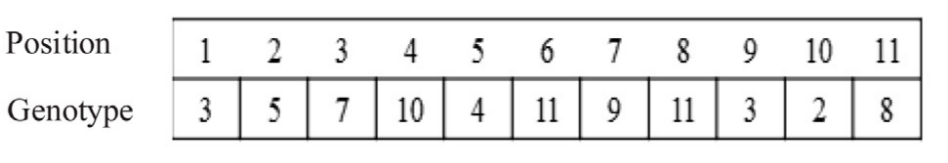
\includegraphics[width=0.6\textwidth]{locus.png}
\caption{The locus representation of a graph.}\label{figure:locus}
\end{center}
\end{figure}

An individual is represented as an array of numbers. 
The index represents the identification number of a vertice in the graph.
The value in the array stands for the vertice it is connected to.
While decoding the representation we say that a set of vertices are in a group if there is a link between any of the vertices.

\begin{figure}
\begin{center}
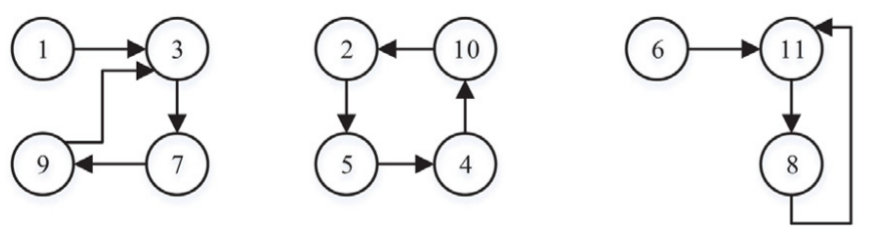
\includegraphics[width=0.6\textwidth]{encode.png}
\caption{The visualisation of Fig. \ref{figure:locus}.}\label{figure:encode}
\end{center}
\end{figure}

\subsubsection{Operators}
The goal of the algorithm is to improve on the initial population which can be initiated randomly or with a heuristic.
To do so some operators are required.
Exploring the search space in usually done by using mutation which will randomly change an individual.
Exploitation is done by combining information of two (or more) individuals to one (or more) new individual(s).
For both of these a short explanation will be given.
\newpage
\subsubsection*{Crossover}
Crossover is the operator that will take care of find the optimum in the current population by combining high scoring individuals with eachother.
By doing this an attempt to select the superior parameters will be taken from both and used to form an even better individual to the problem.
Combining two good solutions doesn't always lead to a better one, but combining one good solution with a bad one might do so.

Some example of crossovers on binary representations are the following:
\begin{itemize}
\item In one-point crossover a random crossover point is selected. All of the information on the left side of the first individual will be combined with the information on the right side of this point of the second individual. A simple example of this can be seen below.
\begin{center}
\begin{tabular}{|c|c|c|c|c|c|}
\hline
0 & 1 & 0 & \textbf{0} & \textbf{0} & \textbf{1} \\ \hline \hline
0 & 1 & 0 & \textbf{1} & \textbf{1} & \textbf{0} \\ \hline
\end{tabular}
\\
$\downarrow$
\\
\begin{tabular}{|c|c|c||c|c|c|}
\hline
0 & 1 & 0 & \textbf{1} & \textbf{1} & \textbf{0} \\ \hline \hline
0 & 1 & 0 & \textbf{0} & \textbf{0} & \textbf{1} \\ \hline
\end{tabular}
\end{center}
\item In two-point crossover two random crossover points are selected. All of the information between these two points will be exchanged between the two individuals. Again a simple example is shown here.
\begin{center}
\begin{tabular}{|c|c|c|c|c|c|}
\hline
1 & 0 & \textbf{1} & \textbf{1} & 0 & 0 \\ \hline \hline
0 & 1 & \textbf{0} & \textbf{1} & 1 & 0 \\ \hline
\end{tabular}
\\
$\downarrow \qquad \quad \downarrow$
\\
\begin{tabular}{|c|c||c|c||c|c|}
\hline
1 & 0 & \textbf{0} & \textbf{1} & 0 & 0 \\ \hline \hline
0 & 1 & \textbf{1} & \textbf{1} & 1 & 0 \\ \hline
\end{tabular}
\end{center}
\end{itemize}

The probability of crossover is in practice chosen quite high, because this is the main exploiting operator.
Without crossover it seems to be very difficult to keep improving on the current population.

\subsubsection*{Mutation}
Mutation normally allows for new sections of the search space to be explored by creating a new value for a parameter that previously wasn't present in the population.
An expample of this is a bit flip on a binary representation for a possible solution.
By doing this a bit that is always $0$ in the population can be changed to $1$ and thus introducing new ``DNA'' into the population.
This is necessary to keep the population from going into a local optima instead of exploring the entire search space and potentially missing out on a better solution. \\

\begin{center}
\begin{tabular}{|c|c|c|c|c|c|}
\hline
1 & 0 & \textbf{1} & 1 & 0 & 0 \\ 
\hline
\end{tabular}
\\
$\quad \downarrow \: \qquad \:$
\\
\begin{tabular}{|c|c|c|c|c|c|}
\hline
1 & 0 & \textbf{0} & 1 & 0 & 0 \\ \hline
\end{tabular}
\end{center}

In practice the amount of mutations is randomly chosen as well as the bits that are being flipped.
The example shows only a single bit flip.
Probablity of a mutation happening is normally chosen quite low as it can disrupt the current exploitation process.